\chapter{AND vs OR Decomposition}
\label{chap:and-vs-or}
As we defined the \orDecomp as a conceptual counterpart to the \andDecomp, we considered different \DFAs with either a \andDecomp or an \orDecomp. Of course there exist \DFAs with both and- and \orDecomp but we try to prove that this is not the case for every \DFA. For an example see Figures \ref{fig:factors-and-example} and \ref{fig:factors-or-example}, where $A$ has a \andDecomp and $B$ has a \orDecomp but not vice versa.

\begin{figure}[h]
	\begin{minipage}[t]{\textwidth}
		\centering
		\begin{tikzpicture}[shorten >=1pt,node distance=2cm,on grid,auto] 
			\node[state,initial] (q_0)   {$q_0$}; 
			\node[state,accepting] (q_1) [ right=of q_0] {$q_1$}; 
			\node[state] (q_2) [ right=of q_1] {$q_2$}; 
			\node[state,accepting] (q_3) [ right=of q_2] {$q_3$};
			\node[state](q_4) [ right=of q_3] {$q_4$};
			\node[state](q_5) [ right=of q_4] {$q_5$};
			\path[->] 
			(q_0) edge  node {} (q_1)
			(q_1) edge  node {} (q_2)
			(q_2) edge  node {} (q_3)
			(q_3) edge  node {} (q_4)
			(q_4) edge  node {} (q_5)
			(q_5) edge[bend right, above]  node {} (q_0);
		\end{tikzpicture}		
	\end{minipage}
	\begin{minipage}[b]{0.39\textwidth}
		\centering
		\begin{tikzpicture}[shorten >=1pt,node distance=2cm,on grid,auto] 
			\node[state,initial] (q_0)   {$q_0$}; 
			\node[state,accepting] (q_1) [right=of q_0] {$q_1$}; 
			\path[->] 
			(q_0) edge  node {} (q_1)
			(q_1) edge[bend right, above]  node {} (q_0);
		\end{tikzpicture}
	\end{minipage}
	\begin{minipage}[b]{0.59\textwidth}
		\centering
		\begin{tikzpicture}[shorten >=1pt,node distance=2cm,on grid,auto] 
			\node[state,initial,accepting] (q_0)   {$q_0$}; 
			\node[state,accepting] (q_1) [right=of q_0] {$q_1$}; 
			\node[state](q_2) [right=of q_1] {$q_2$};
			\path[->] 
			(q_0) edge  node {} (q_1)
			(q_1) edge  node {} (q_2)
			(q_2) edge[bend right, above]  node {} (q_0);
			
		\end{tikzpicture}
	\end{minipage}
	\caption{The DFA $A$ and its factor $A_2$ and $A_3$ (and-decomposition)}
	\label{fig:factors-and-example}
\end{figure}

\begin{figure}[h]
	\begin{minipage}[t]{\textwidth}
		\centering
		\begin{tikzpicture}[shorten >=1pt,node distance=2cm,on grid,auto] 
			\node[state,initial] (q_0)   {$q_0$}; 
			\node[state,accepting] (q_1) [ right=of q_0] {$q_1$}; 
			\node[state] (q_2) [ right=of q_1] {$q_2$}; 
			\node[state,accepting] (q_3) [ right=of q_2] {$q_3$};
			\node[state,accepting](q_4) [ right=of q_3] {$q_4$};
			\node[state,accepting] (q_5) [ right=of q_4] {$q_5$};
			\path[->] 
			(q_0) edge  node {} (q_1)
			(q_1) edge  node {} (q_2)
			(q_2) edge  node {} (q_3)
			(q_3) edge  node {} (q_4)
			(q_4) edge  node {} (q_5)
			(q_5) edge[bend right, above]  node {} (q_0);
		\end{tikzpicture}		
	\end{minipage}
	\begin{minipage}[b]{0.39\textwidth}
		\centering
		\begin{tikzpicture}[shorten >=1pt,node distance=2cm,on grid,auto] 
			\node[state,initial] (q_0)   {$q_0$}; 
			\node[state,accepting] (q_1) [right=of q_0] {$q_1$}; 
			\path[->] 
			(q_0) edge  node {} (q_1)
			(q_1) edge[bend right, above]  node {} (q_0);
			
		\end{tikzpicture}
	\end{minipage}
	\begin{minipage}[b]{0.59\textwidth}
		\centering
		\begin{tikzpicture}[shorten >=1pt,node distance=2cm,on grid,auto] 
			\node[state,initial] (q_0)   {$q_0$}; 
			\node[state,accepting] (q_1) [right=of q_0] {$q_1$}; 
			\node[state](q_2) [right=of q_1] {$q_2$};
			\path[->] 
			(q_0) edge  node {} (q_1)
			(q_1) edge  node {} (q_2)
			(q_2) edge[bend right, above]  node {} (q_0);
			
		\end{tikzpicture}
	\end{minipage}
	\caption{The DFA $B$ and its factors $B_2$ \& $B_3$ (or-decomposition)}
	\label{fig:factors-or-example}
\end{figure}

To prove that there exists words which are and-decomposable but not or-decomposable and vice versa, we need a bit of background. For this purpose we have:

\begin{lemma}
	$$ w  = A \land B = \overbar{\overbar{A} \lor \overbar{B}}$$
\end{lemma}

\begin{theorem}
	$$ \exists ~w~ \text{s.t.} ~w~ \text{is and-decomposable but not or-decomposable}$$
\end{theorem}

\begin{proof}
	Assume $\overbar{w}$ is not and-decomposable and $w = v_1 \lor v_2 \lor \dots \lor v_k$. Using the Lemma 1, we obtain $w = \overbar{\overbar{v_1} \land \overbar{v_2} \land \dots \land \overbar{v_k}}$ which is equal to $\overbar{w} = \overbar{v_1} \land \overbar{v_2} \land \dots \land \overbar{v_k}$. This implies $w$ is not or-decomposable via contradiction.
\end{proof}


\begin{theorem}
	$$ \exists ~w~ \text{s.t.} ~w~ \text{is or decomposable but not and-decomposable}$$
\end{theorem}

\begin{corollary}
	The Set of or-decomposable strings and the set of and-decomposable string is not comparable.
\end{corollary}

\begin{figure}[h]
	\centering
	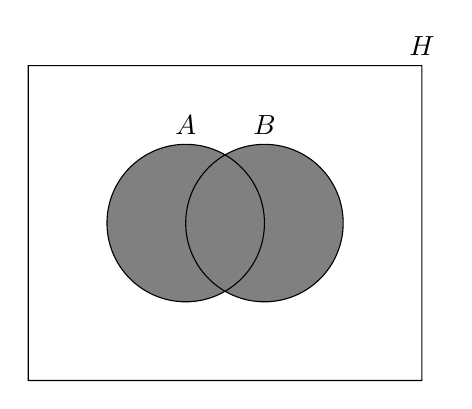
\begin{tikzpicture}[fill=gray]
		% left hand
		\scope
		\clip (-2,-2) rectangle (2,2)
		(1,0) circle (1);
		\fill (0,0) circle (1);
		\endscope
		% right hand
		\scope
		(0,0) circle (1);
		\fill (1,0) circle (1);
		\endscope
		% outline
		\draw (0,0) circle (1) (0,1)  node [text=black,above] {$A$}
		(1,0) circle (1) (1,1)  node [text=black,above] {$B$}
		(-2,-2) rectangle (3,2) node [text=black,above] {$H$};
	\end{tikzpicture}
\label{fig:set-of-and-and-or-decomposable-words}
\caption{TODO}
\end{figure}

%%% Local Variables: 
%%% mode: latex
%%% TeX-master: "thesis"
%%% End: 